\chapter{Modely simultánních rovnic}

V předchozí kapitole jsme se zaobírali nezávislou proměnnou, která je korelovaná s chybovým členem. Takovouto veličinu jsme označili za endogenní. Další důležitá forma endogenity nezávislých proměnných má podobu tzv. simultánnosti. Ta nastává, jestliže je jedna nebo vícero nezávislých veličin ustanovena společně se závislou veličinou typicky skrze model popisující dosažení bodu rovnováhy. Tyto modely nazýváme modely simultánních rovnic [simultaneous equation models (SEMs)]. Hlavní metodou pro odhad těchto modelů je metoda pomocných veličin.

\section{Podstata modelů simultánních rovnic}

Důležitým vodítkem při formulování SEM je, že každá rovnice by měla mít ekonomickou interpretaci. Klasickým příkladem SEM jsou modely nabídky a poptávky. Pro ilustraci uvažujme trh práce v zemědělství pro určitý kraj. Jednoduchou rovnici nabídky práce můžeme definovat jako
\begin{equation}
h_s = \alpha_1 w + \beta_1 z_1 + u_1,
\end{equation}
kde $h_s$ představuje objem nabízené práce v hodinách, $w$ představuje hodinou mzdu v zemědělství a $z_1$ hodinovou mzdu ve zpracovatelském průmyslu. Rovnice (16.1) je strukturální rovnicí. Toto označení odráží skutečnost, že (16.1) vychází ekonomické teorie a lze ji poměrně jednoduše interpretovat. Pro veličinu $z_1$ se někdy používá označení pozorovaná veličina posunu nabídky (observed supply shifter) a pro veličinu $u_1$ označení nepozorovaná veličina posunu nabídky (unobserved supply shifter).

Rovnice (16.1) by měla popisovat nabídku práce pro všechny možné úrovně mezd nabízených v zemědělství a ve zpracovatelském průmyslu. Bohužel však v praxi není možné pro jednotlivé kraje nastavit různé úrovně mezd, pro které bychom následně zkoumali objem nabízené práce. Proto nemůžeme model odhadnout pomocí OLS. Abychom pochopili vztah mezi úrovní mezd a objemem nabízené práce, musíme uvažovat model, který bude popisovat vzájemnou interakci mezi nabídkou a poptávkou na trhu práce s cílem získat bod rovnováhy, tj. bod, ve které je objem nabízené práce roven objemu poptávané práce. Jinými slovy potřebujeme definovat rovnici popisující poptávku po práci. Pro tento účel můžeme použít např. model
\begin{equation}
h_d = \alpha_2 w + \beta_2 z_2 + u_2,
\end{equation}
$h_d$ označuje poptávku po práci v hodinách, $w$ opět představuje hodinovou mzdu a $z_2$ je rozloha zemědělské půdy v kraji. Výše představenou terminologií tak $z_2$ představuje pozorovanou veličinu posunu nabídky a $u_1$ nepozorovanou veličinu posunu nabídky. Stejně jako v případě (16.1) i (16.2) je strukturální rovnicí.

Rovnice (16.1) popisuje chování strany nabídky a (16.2) chování strany poptávky na trhu práce. Rovnovážná mzda je pak dána průsečíkem nabídky a poptávky, tj.
\begin{equation}
h_{is} = h_{id}.
\end{equation}
Pokud s pomocí (16.3) zkombinujeme (16.1) a (16.2), získáme
\begin{equation}
h_i = \alpha_1 w_i + \beta_1 z_{i1} + u_{i1}
\end{equation}
a
\begin{equation}
h_i = \alpha_2 w_i + \beta_2 z_{i2} + u_{i2}.
\end{equation}
Tyto dvě rovnice definují SEM. Pro dané $z_{i1}$, $z_{i2}$, $u_{i1}$ a $u_{i2}$ jsme s jejich pomocí schopni určit $h_1$ a $w_i$.\footnote{Navíc musíme předpokládat $\alpha_1 \ne \alpha_2$. Nicméně z ekonomické teorie poměrně jasně vyplývá, že $\alpha_1 > 0$ a $\alpha_2 < 0$, takže lze tuto podmínku považovat za splněnou.} Z tohoto důvodu jsou $h_i$ a $w_i$ v tomto modelu endogenními veličinami. Naproti tomu $z_{i1}$ a $z_{i2}$ jsou exogenními veličinami, protože jsou určeny mimo systém rovnic (16.4) a (16.5). Základním předpokladem je, že $z_{i1}$ a $z_{i2}$ jsou nekorelované s $u_{i1}$ a $u_{i2}$, které označujeme jako strukturálních chybové členy (structural errors), protože figurují ve strukturálních rovnicích.

Bez zahrnutí $z_1$ a $z_2$ do modelu simultánních rovnic nejsme schopni rozlišit funkci nabídky a funkci poptávky. Pokud $z_1$ představuje náklady obětované příležitosti ve formě mzdy ve zpracovatelském průmyslu, pak rovnice obsahující $z_1$ je funkcí nabídky práce. Analogickou argumentaci lze použít také v případě rovnice obsahující veličinu $z_2$, která představuje rozlohu zemědělské půdy v kraji. Pokud by $z_1$ a $z_2$ byly totožné - např. průměrná úroveň vzdělání v kraji, která může ovlivňovat jak stranu nabídky, tak stranu poptávky - pak by obě rovnice byly totožné a nebyli bychom schopni odhadnout žádnou z nich.

SEM mají nejčastěji podobu výše uvedeného modelu nabídky a poptávky. Ne vždy je však jednoduché správně rozhodnout, kdy je použití SEM vhodné. Příkladem takovéto špatné aplikace je modelování počtu hodin, které týdně strávíme studiem a prací. Jenom proto, že jsou dvě veličiny odhadovány současně, neznamená, že bychom měli aplikovat model simultánních rovnic. Ten je vhodné aplikovat pouze tehdy, kdy mají obě rovnice samy o sobě ekonomickou interpretaci. V případě počtu hodin strávených studiem a prací tento předpoklad splněn není.

\section{Zkreslení OLS}

V jednoduchém modelu, ve kterém je nezávislá veličina určena současně se závislou veličinou, je tato veličina korelována s chybovým členem, což má za následek zkreslení OLS odhadů. Pro ilustraci uvažujme model
\begin{equation}
y_1 = \alpha_1 y_2 + \beta_1 z_1 + u_1
\end{equation}
\begin{equation}
y_2 = \alpha_2 y_1 + \beta_2 z_2 + u_2.
\end{equation}
Veličiny $z_1$ a $z_2$ jsou exogenní, a proto jsou nekorelované s $u_1$ a $u_2$. Spojením obou rovnic získáváme
\begin{equation}
y_2 = \alpha_2 (\alpha_1 y_2 + \beta_1 z_1 + u_1) + \beta_2 z_2 + u_2,
\end{equation}
což lze dále upravit na
\begin{equation}
(1 - \alpha_2 \alpha_1)y_2 = \alpha_2 \beta_1 z_1 + \beta_2 z_2 + \alpha_2 u_1 + u_2
\end{equation}
a následně na
\begin{equation}
y_2 = \pi_{21}z_1 + \pi_{22}z_2 + v_2,
\end{equation}
kde $\pi_{21} = \frac{\alpha_2 \beta_1}{1 - \alpha_2 \alpha_1}$, $\pi_{22} = \frac{\beta_2}{1 - \alpha_2 \alpha_1}$, $v_2 = \frac{\alpha_2 u_1 + u_2}{1 - \alpha_2 \alpha_1}$ za předpokladu splnění podmínky $\alpha_2 \alpha_1 \ne 1$. Rovnici (16.10) nazýváme rovnicí redukované formy (reduced form equation) pro $y_2$ a $\pi_{21}$ a $\pi_{22}$ nazýváme parametry redukované formy. Tyto parametry jsou nelineární funkcí strukturálních parametrů. Chybový člen $v_2$ redukované formy je lineární funkcí strukturálních chybových členů $u_1$ a $u_2$. Protože jsou $u_1$ a $u_2$ nekorelované s $z_1$ a $z_2$, je také $v_2$ nekorelované s $z_1$ a $z_2$. Proto jsme schopni konzistentně odhadnout $\pi_{21}$ a $\pi_{22}$ pomocí OLS.

Při splnění $\alpha_2 \alpha_1 \ne 1$ existuje redukovaná forma také pro $y_1$, která má stejné vlastnosti jako redukovaná forma pro $y_2$.

Na rovnici (16.10) můžeme dokázat, že s výjimkou splnění specifických předpokladů, vede aplikace OLS na (16.6) ke zkresleným a nekonzistentním odhadům $\alpha_1$ a $\beta_1$. Protože $z_1$ a $u_1$ jsou z definice nekorelované, jedinou nezodpovězenou otázkou zůstává, zda-li jsou $y_2$ a $u_1$ rovněž nekorelované. Z redukované formy (16.10) je zřejmé, že $y_2$ a $u_1$ je korelované pouze tehdy a jen tehdy, pokud jsou $v_2$ a $u_1$ korelované.\footnote{Připomeňme, že $z_1$ a $z_2$ jsou exogenní veličiny a tudíž nekorelované s $v_2$.} Protože $v_2$ je lineární funkcí $u_1$  a $u_2$, je obecně korelováno s $u_1$. Pokud předpokládáme, že $u_1$ a $u_2$ jsou nekorelované, pak $v_2$ a $u_1$ musí být korelované, kdykoliv $\alpha_2 \ne 0$. I kdyby $\alpha_2 = 0$, jsou $v_2$ a $u_1$ korelované, pokud jsou korelované $u_1$ a $u_2$.

Pokud je $y_2$ korelováno s $u_1$ z důvodů simultánnosti, pak říkáme, že OLS trpí simultánním zkreslením. Zjištění směru tohoto zkreslení je v případě obecného modelu komplikované, což jsme ostatně ilustrovali na příkladech v kapitolách 3 a 5. V případě jednoduchého modelu to však možné je. Předpokládejme, že z rovnice (16.6) vynecháme $z_1$ a dále předpokládejme, že $u_1$ a $u_2$ jsou nekorelované. Pak je kovariance mezi $y_2$ a $u_1$ dána
\begin{equation}
cov(y_2, u_1) = cov(v_2, u_1) = \frac{\alpha_2}{1 - \alpha_2 \alpha_1}E[u^2_1] = \frac{\alpha_2}{1 - \alpha_2 \alpha_1} \sigma_1^2,
\end{equation}
kde $\sigma_1^2 = var[u_1] > 0$. Proto má asymptotické zkreslení OLS odhadu pro $\alpha_1$ stejné znaménko jako $\frac{\alpha_2}{1 - \alpha_2 \alpha_1}$.

\section{Formulace a odhad strukturální rovnice}

\subsection{Formulace strukturální rovnice}

Při odhadování modelu pomocí OLS je klíčové, aby každá vysvětlující veličina byla nekorelovaná s chybovým členem. Jak jsme dokázali v předchozí kapitole, není tento předpoklad splněn v případě obecných SEM. Nicméně pokud máme pomocné veličiny, můžeme konzistentně odhadnout parametry tohoto modelu a to podobným způsobem jako v případě opominuté veličiny nebo chyby měření.

Uvažujme jednoduchý model nabídky a poptávky s bodem rovnováhy $q = q_s = q_d$ definovaným jako
\begin{equation}
q = \alpha_1 p + \beta_1 z_1 + u_1
\end{equation}
a
\begin{equation}
q = \alpha_2 p + u_2.
\end{equation}
Předpokládejme, že $q$ představuje spotřebu mléka na obyvatele v kraji, $p$ průměrnou cenu za litr mléka v kraji a $z_1$ je cena krmiva a představuje tak exogenní veličinu. Vzhledem k $z_1$ je tedy zřejmé, že (16.12) představuje funkci nabídky a (16.13) funkci poptávky.\footnote{Cena krmiva pro dobytek zcela zřejmě ovlivňuje stranu nabídky, nikoliv poptávky.} 

Otázkou zůstává, kterou rovnici můžeme pro náhodný výběr $(q, p, z_1)$ odhadnout, tj. která z těchto rovnic je identifikovaná (identified equation). Identifikovanou rovnicí je rovnice poptávky (16.13); rovnice nabídky (16.12) identifikovaná není. Důvodem je, že ačkoliv můžeme $z_1$ použít jako pomocnou veličinu pro cenu mléka v rovnici (16.13), nemůžeme ji použít jako pomocnou veličinu také v rovnici (16.12), protože zde již figuruje jako nezávislá veličina.

Pokud by byl chybový člen $u_2$ nulový, byli bychom s pomocí $z_1$ schopni identifikovat funkci poptávky tak, jak je ilustrováno následujícím obrázkem. Přítomnost $u_2$ má však za následek to, že jsme schopni odhadnout funkci poptávky pouze s chybou, nicméně odhady jejích parametrů budou konzistentní, pokud je $z_1$ nekorelované s $u_2$. Funkci nabídky nejsme schopni identifikovat, protože pro ni neexistují žádné pozorované veličiny, které by mohly figurovat v roli veličiny posunu.
\begin{figure}[htp]
\centering
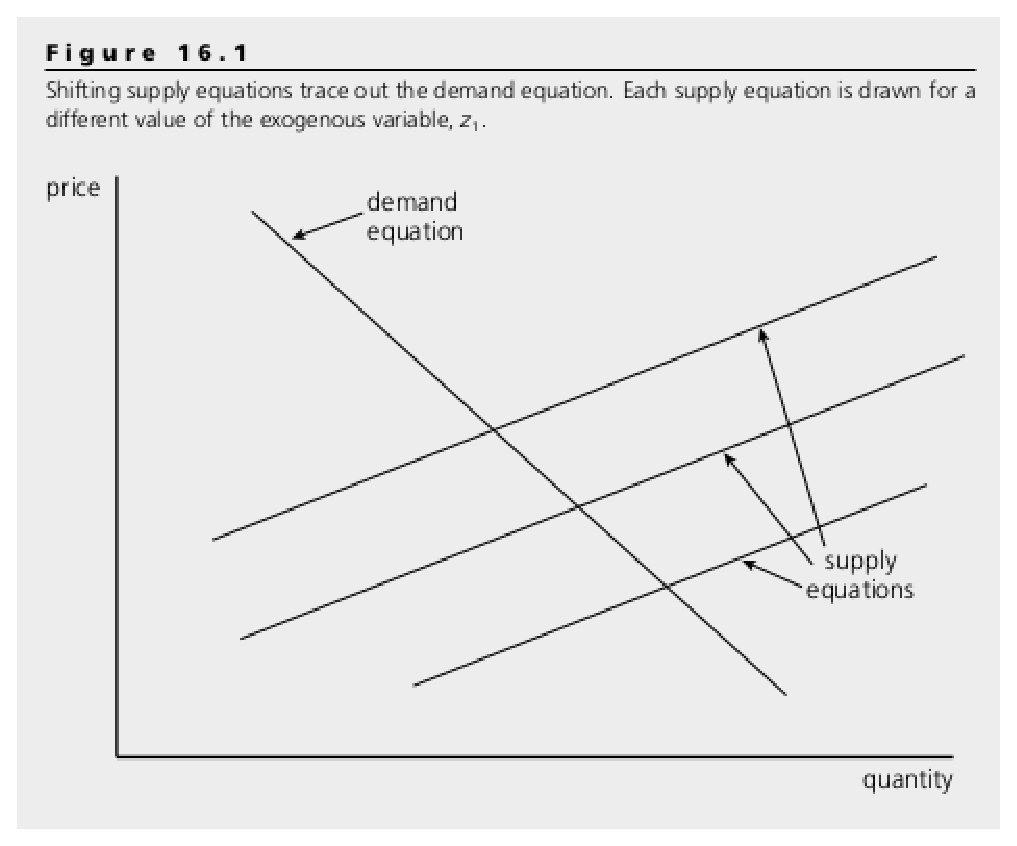
\includegraphics[scale = 0.5]{pictures/figure_16_1.eps}
\caption{Identifikace funkce poptávky pomocí $z_1$}
\label{figure_16_1}
\end{figure}

Rozšíření myšlenky identifikace na obecný případ modelu o dvou rovnicích je poměrně přímočaré. Uvažujme rovnice
\begin{equation}
y_1 = \beta_{10} + \alpha_1 y_2 + \pmb{z}_1 \pmb{\beta}_1 + u_1
\end{equation}
a
\begin{equation}
y_2 = \beta_{20} + \alpha_2 y_1 + \pmb{z}_2 \pmb{\beta}_2 + u_2,
\end{equation}
kde $y_1$ a $y_2$ jsou endogenní veličiny a $u_1$ a $u_2$ jsou strukturální chybové členy. Dále $\pmb{z}_1$ představuje vektor $k_1$ exogenních veličin figurujících v první rovnici, tj. $\pmb{z}_1 = (z_{11}, z_{12}, ..., z_{1 k_1})$. Podobně $\pmb{z}_2$ představuje vektor $k_2$ exogenních veličin obsažených v druhé rovnici, tj. $\pmb{z}_2 = (z_{21}, z_{22}, ..., z_{2 k_2})$. V mnoha případech se budou $\pmb{z}_1$ a $\pmb{z}_2$ překrývat. Nicméně je nutné, aby se tyto dva vektory nepřekrývaly zcela.\footnote{To by mimo jiné znamenalo, že nejsme schopni od sebe tyto rovnice odlišit.}

Rovnice (16.14) a (16.15) můžeme řešit s ohledem na $y_1$ a $y_2$, pokud je splněna podmínka $\alpha_2 \alpha_1 \ne 1$. Důkaz je ve své podstatě identický s příkladem jednoduchého modelu, který jsme představili v kapitole 16.2. Při splnění této podmínky existuje redukovaná forma pro $y_1$ i $y_2$.

\subsubsection{Podmínka identifikace}

První z SEM rovnic v modelu o dvou rovnicích je identifikovaná pouze tehdy a jen tehdy, pokud druhá rovnice obsahuje alespoň jednu exogenní veličinu (s nenulovým koeficientem), která není součástí této první rovnice. Tuto podmínku je možné otestovat pomocí $t$ popř. $F$ statistiky stejně, jak jsme si ukázali v kapitole 15.

\subsection{Odhad pomocí 2SLS}

Pokud je daná rovnice identifikovaná, můžeme ji odhadnout pomocí metody 2SLS. Pomocné veličiny se ``rekrutují'' z exogenních veličin, které figurují v některé z SEM rovnic.

\section{Simultánní modely s více než dvěma rovnicemi}

SEM mohou zahrnovat více než dvě rovnice. Obecná analýza těchto modelů je složitá a vyžaduje lineární algebru. V okamžiku, kdy je některá z rovnic identifikována, může být odhadnuta pomocí metody 2SLS.

\subsection{Model se třemi rovnicemi}

Pro ilustraci uvažujme následující systém rovnic.
\begin{equation}
y_1 = \alpha_{12}y_2 + \alpha_{13}y_3 + \beta_{11}z_1 + u_1
\end{equation}
\begin{equation}
y_2 = \alpha_{21} y_1 + \beta_{21}z_1 + \beta_{22}z_2 + \beta_{23}z_3 + u_2
\end{equation}
\begin{equation}
y_3 = \alpha_{32} y_2 + \beta_{31}z_1 + \beta_{32}z_2 + \beta_{33}z_3 + \beta_{34}z_4 + u_3
\end{equation}
Jako obvykle $y_g$ představuje endogenní veličiny a $z_j$ pak exogenní veličiny. První dolní index označuje číslo rovnice a druhý dolní index pak číslo veličiny. Parametry endogenních veličin označujeme jako $\alpha$ a parametry exogenních veličin jako $\beta$.

Kterou z výše uvedených rovnic můžeme odhadnout pomocí metody 2SLS? V případě obecného SEM s vícero rovnicemi je velmi problematické určit identifikovanou rovnici. Nicméně je mnohdy poměrně jednoduché určit neidentifikované rovnice. V případě výše uvedeného modelu je zřejmé, touto neidentifikovanou rovnicí je rovnice (16.18). Protože je v této rovnici obsažena každá exogenní veličina, nezůstává žádná exogenní veličina, kterou bychom mohli použít pro $y_2$ v roli pomocné veličiny. Proto nemůžeme konzistentně odhadnout parametry této rovnice. Rovnice (16.16) naproti tomu vypadá slibně - tato rovnice neobsahuje exogenní veličiny $z_2$, $z_3$ ani $z_4$, které tak mohou být použity jako pomocné veličiny. Ačkoliv (16.16) zahrnuje dvě endogenní veličiny, máme k dispozici tři exogenní veličiny, které můžeme použít jako pomocné veličiny pro $y_2$ a $y_3$. Rovnice (16.17) také vypadá slibně, protože exogenní veličinu $z_4$, která není v této rovnici obsažena, můžeme použít jako pomocnou veličinu pro jedinou endogenní veličinu $y_1$.

Obecná podmínka tedy zní, že pro danou rovnici musíme mít k dispozici alespoň tolik ``nevyužitých'' exogenních veličin jako je počet endogenních veličin zahrnutých v této rovnici. Tato podmínka je však nutná, nikoliv postačující pro identifikaci rovnice. Pokud by např. $\beta_{34} = 0$, pak $z_4$ nefiguruje v žádné ze tří rovnic simultánního modelu, což znamená, že není korelovaná s $y_1$, $y_2$ ani s $y_3$. Druhá rovnice tak není identifikována, protože $z_4$ nemůže být použita jako pomocná veličina pro $y_1$. To, zda-li je daná rovnice identifikována, tak záleží na hodnotách parametrů ostatních rovnic.

V souvislosti s identifikací rovnic se často setkáme s pojmy přeidentifikovaná rovnice (overidentified equation), právě identifikovaná rovnice (just identified equaiton) a neidentifikovaná rovnice (unidentified equaiton). Pojem přeidentifikovaná rovnice popisuje situaci, kdy je počet ``nevyužitých'' exogenních veličin vyšší než počet endogenních veličin zahrnutých do rovnice. V našem ilustrativním příkladě je tak rovnice (16.16) přeidentifikovanou rovnicí. Právě identifikovaná rovnice je pak rovnice, pro kterou je počet ``nevyužitých'' exogenních veličin roven endogenních veličin. Příkladem této rovnice je rovnice (16.17). V případě neidentifikované rovnice je pak počet ``nevyužitých'' exogenních veličin menší než počet endogenních veličin obsažených v rovnici. V našem případě se jedná o rovnici (16.18).

\subsection{Odhad}

Bez ohledu na počet rovnic v simultánním modelu je možné každou identifikovanou rovnici odhadnout pomocí metody 2SLS. Množinu potenciálních pomocných veličin představují všechny exogenní veličiny, které jsou zahrnuty v libovolné rovnici modelu. Testy pro endogenitu, heteroskedasticitu, autokorelaci a nadbytečnou identifikaci lze zkonstruovat způsobem popsaným v kapitole 15.

\section{Simultánní model a časové řady}

Mezi historicky první aplikace SEM patří modely popisující vývoj ekonomiky. Jako příklad uvažujme jednoduchý Keynesiánský model agregované poptávky ve tvaru
\begin{equation}
C_t = \beta_0 + \beta_1 (Y_t - T_t) + \beta_2 r_t + u_{t1}
\end{equation}
\begin{equation}
I_t = \gamma_0 + \gamma_1 r_t + u_{t2}
\end{equation}
\begin{equation}
Y_t \equiv C_t + I_t + G_t,
\end{equation}
kde $C_t$ představuje spotřebu, $Y_t$ příjem, $T_t$ daňové odvody, $r_t$ úrokovou sazbu, $I_t$ investice a $G_t$ vládní výdaje. Předpokládáme, že $t$ označuje rok.

První rovnice představuje funkci agregované spotřeby, která závisí na disponibilním příjmu $Y_t - T_t$, úrokové sazbě a strukturálním chybovém členu $u_{t1}$. Druhá rovnice představuje jednoduchou funkci investic. Poslední rovnice je identitou, která je dána metodikou národního účetnictví. Tato rovnice platí z definice a tudíž neobsahuje chybový člen. Rovnici (16.21) neodhadujeme, nicméně ji potřebuje pro úplnou definici modelu.

Protože je náš model definován třemi rovnicemi, musí se v něm vyskytovat také tři endogenní veličiny. Při pohledu na první dvě rovnice je patrné, že $C_t$ a $I_t$ jsou zamýšleny jako endogenní veličiny. Navíc, s ohledem na výše uvedenou účetní identitu, je $Y_t$ třetí endogenní veličinou. V rámci modelu pak předpokládáme, že $T_t$, $r_t$ a $G_t$ jsou exogenní veličiny a jsou tak nekorelované s $u_{t1}$ a $u_{t2}$.

Pokud je $r_t$ exogenní, můžeme (16.20) odhadnout pomocí OLS. Funkce spotřeby závisí na disponibilním příjmu $Y_t - T_t$, který je endogenní, protože $Y_t$ je endogenní. K dispozici však máme dvě exogenní veličiny $T_t$ a $G_t$. Tuto rovnici tak jsme schopni odhadnout pomocí 2SLS a pomocných proměnných $(T_t, G_t, r_t)$.

Problémem výše uvedeného SME je jeho statičnost. To se však dá snadno napravit zahrnutím zpožděných veličin. Např. rovnici (16.20) lze upravit na
\begin{equation}
I_t = \gamma_0 + \gamma_1 r_t + \gamma_2 Y_{t - 1} + u_{t2}
\end{equation}
Můžeme v tomto kontextu chápat $Y_{t-1}$ jako exogenní veličinu? Při splnění určitých předpokladů ohledně $u_{t2}$ ano. Nicméně obvykle nazýváme zpožděnou endogenní veličinu zahrnutou do simultánního modelu jako předvybranou veličinou (predetermined variable). Jestliže předpokládáme, že $u_{t2}$ je nekorelované se současnými exogenními veličiny a všemi minulými endogenními a exogenními veličinami, pak je $Y_{t-1}$ z definice nekorelované s $u_{t2}$. S ohledem na exogenitu $r_t$ tak můžeme (16.22) odhadnout pomocí OLS.

Pokud bychom přidali $C_{t-1}$ do (16.19), můžeme tuto zpožděnou veličinu považovat za exogenní za předpokladu, že je nekorelované s $u_{t1}$. Tím získáme následující rovnici.
\begin{equation}
C_t = \beta_0 + \beta_1 (Y_t - T_t) + \beta_2 r_t + \beta_3 C_{t - 1} + u_{t1}
\end{equation}
Protože je současný disponibilní příjem $(Y_t - T_t)$ je stále endogenní, musíme tuto rovnici odhadnout pomocí 2SLS s využitím pomocným veličin $(T_t, G_t, r_t, C_{t-1})$. Pokud je funkce investic dána (16.22), pak může být na list pomocných veličin přidána také veličina $I_{t-1}$.

Platnost klasické OLS a 2SLS metody pro účely určení konfidenčních intervalů, $t$ a $F$ testů závisí na předpokladu slabé závislosti. Bohužel makroekonomické veličiny velmi často tento předpoklad porušují. Terminologií kapitoly 11 je označujeme jako proces s jednotkovým kořenem. Dokonce i ve výběrech velkého rozsahu (nemluvě o výběrech malého rozsahu) jsou vlastnosti OLS a 2SLS odhadů procesů s jednotkovým kořenem komplikované a závisí na celé řadě předpokladů. Problém jednotkového kořene lze alespoň částečně vyřešit pomocí první diference podkladové časové řady. Nicméně je třeba si uvědomit, že po aplikaci diference se již jedná o jiný model.

Dalším praktickým problémem SEM může být nalezení vhodných pomocných veličin. Tento problém je obvykle snadněji řešitelný pro dezagregovaná data. Jako příklad uvažujme zpracovatelský průmysl, kde výstup jednoho odvětví může být použit jako pomocná veličina pro nabídkovou funkci druhého odvětví.

\section{Panelová data}

Uvažujme situaci, kdy se snažíme odhadnout funkci nabídky práce a funkci nabízené mzdy pro určitou skupinu lidí a určitý časový úsek. Kromě odhadu parametrů pro jednotlivé časové periody můžeme také pro jednotlivé rovnice uvažovat nepozorované veličiny. Např. pro nabídku práce můžeme uvažovat nepozorovanou hodnotu volného času, o které můžeme předpokládat, že je konstantní v čase.

Základní přístup při odhadu simultánního modelu nad panelovými daty zahrnuje dva kroky. Nejprve se pokusíme odstranit nepozorované veličiny (např. konstantní hodnotu volného času) pomocí první diference nebo jiné vhodné transformace. Následně najdeme vhodné pomocné veličiny pro endogenní veličiny zahrnutých v těchto transformovaných rovnicích. Pro ilustraci uvažujme model
\begin{equation}
y_{it1} = \alpha_1 y_{it2} + \pmb{z}_{it1} \pmb{\beta}_1 + a_{i1} + u_{it1}
\end{equation}
\begin{equation}
y_{it2} = \alpha_2 y_{it1} + \pmb{z}_{it2} \pmb{\beta}_2 + a_{i2} + u_{it2},
\end{equation}
kde $i$ označuje průřez (např. konkrétního jedince), $t$ označuje čas a $\pmb{z}_{it1} \pmb{\beta}_1$ popř. $\pmb{z}_{it2} \pmb{\beta}_2$ označují lineární kombinace exogenních nezávislých veličin v jednotlivých rovnicích. V obecném modelu mohou být nepozorované veličiny $a_{i1}$ a $a_{i2}$ korelované se všemi nezávislými veličinami. Nicméně předpokládáme, že idiosynkratické strukturální chybové členy $u_{it1}$ a $u_{it2}$ jsou nekorelované se $\pmb{z}$, což činí $\pmb{z}$ vektorem exogenních veličin. S výjimkou speciálních případů je pak $y_{it2}$ korelováno s $u_{it1}$ a $y_{it1}$ je korelováno s $u_{it2}$.

Předpokládejme, že chceme odhadnout rovnici (16.24). Tuto rovnici však nemůžeme odhadnout pomocí OLS, protože složený chybový člen $a_{i1} + u_{it1}$ je potenciálně korelovaný se všemi nezávislými veličinami. Proto aplikujeme první diferenci, čímž získáme
\begin{equation}
\Delta y_{it1} = \alpha_1 \Delta y_{it2} + \Delta \pmb{z}_{it1} \pmb{\beta}_1 + \Delta u_{it1}.
\end{equation}
Chybový člen v této rovnici je nekorelovaný s $\Delta \pmb{z}_{it1}$, což je dáno našimi výchozími předpoklady. Nicméně $\Delta y_{it2}$ a $\Delta u_{it1}$ jsou stále potenciálně korelované. Proto potřebujeme pomocnou veličinu pro $\Delta y_{it2}$. Pokud bychom aplikovali první diferenci také na (16.25), pak jsou přirozenými pomocnými veličinami pro $\Delta y_{it2}$ veličiny $\Delta \pmb{z}_{it2}$, které nejsou obsaženy v $\Delta \pmb{z}_{it1}$. Aby byl daný prvek $\Delta \pmb{z}_{it2}$ použitelný jako pomocná veličina, musí se měnit v čase. Pokud bych chtěli např. použít veličinu $\Delta exper_{it}$ (změna pracovní praxe v letech), zjistili bychom, že tato veličina není použitelná. Protože všichni jedinci v populaci pracují po celé zkoumané období, platí pro každého z nich v každém roce $\Delta exper_{it} = 1$. Je zřejmé, že takováto veličina je bezcenná.

Testování AR(1) potenciálně přítomné v $r_{it1} = \Delta u_{it1}$ je jednoduché. Nejprve pomocí 2SLS získáme odhad chybového členu $\hat{r}_{it1}$. Následně přidáme chybový člen zpožděný o jednu časovou periodu do původní rovnice, kterou opět odhadneme pomocí 2SLS; $\hat{r}_{it1}$ slouží jako pomocná veličina sebe sama. Autokorelaci lze pak otestovat pomocí obvyklé 2SLS $t$ statistiky aplikované na koeficient zpožděného chybového členu.